
\section{Concepts et utilisation}

Nous allons à présent voir comment fonctionne en détail le protocole IPv4,
autant dans sa partie conceptuelle (paquet, adresse IP, classe d'adresse,
masque de sous-réseau,...) que dans sa partie applicatif (entête IP, routage,
...).

Des données transmisent en utilisant le protocole IPv4 sont encapsulées dans un message que
l'on appelle un paquet IPv4. Ces paquets sont constitués d'un entête suivis des données à transmettre.

% Mossi
\subsection{Adresse IPv4}

L'entête contient des informations essentielles pour la transmission d'un paquet, notamment les
adresses source et destination.

Une adresse IP sert à identifier une machine (et plus précisément une des interfaces de cette machine)
dans un réseau particulier.
Comme nous le verrons plus tard cet identifiant unique permet de désigner à la fois un
réseau et une machine précise au sein de ce réseau.
Une adresse est codé sur 32 bits ce qui permet de coder 2\^32 soit 4294967296 adresses différentes.
Par convention on peut représenter une adresse IPv4 comme une suite de 4 nombres décimaux séparés par des points,
chacun traduisant un octet. Cette représentation a contribué à simplifier l'utilisation et la manipulation
des adresses.
Comme chaque nombre représente un octet, les valeurs de celui-ci sont comprises entre 0 et 255.

\vspace{1cm}
Exemple: adresse à valeur décimale: 212.217.0.1 => correspond sous sa forme
binaire à: 11010100.11011001.00000000.00000001
\vspace{1cm}

\subsubsection{Notion de NET ID et HOST ID}
Une adresse IPv4, en tant qu'identifiant d'une machine dans un réseau, contient deux informations:
une première partie qui identifie le réseau appelé NET ID (les bits de poids fort), une seconde qui identifie l’hôte appeler host-ID (les bits de poids faible).
Les machines qui se trouvent donc sur le même réseau partage le même NET ID pour leur adresse.

La longueur de ces deux parties est variable: la taille du HOST ID dépend de la taille du NET ID. Pour représenter la longueur de ces différentes parties on a introduit la notion de masque

\subsubsection{Masque de réseau}

Le masque sert à représenter la scission entre le NET ID et le HOST ID.
Il est codé sur 32 bits et adopte la même représentation qu'une adresse IP, à savoir
4 nombres décimaux séparé par des points.
La position des bits à 1 dans le masque corresponde à la position des bits définissant le NET ID dans l'adresse IP.
Pour obtenir les bits du NET ID il suffit de faire un ET logique entre l'adresse et son masque. Tous les autres bits (donc les bits à 0)
feront donc partie du HOST ID.
Les bits à 1 sont contiguës et commencent au bit de poids fort: le nombre de bit à 1 dans le masque, donne
le nombre de bit faisant partie du NET ID en partant du bit de poids fort dans l'adresse.

En conséquence plus le nombre de bit à 1 dans le masque est grand, plus le NET ID sera grand, et plus le HOST ID sera petit, car il restera moins de bit pour définir le HOST ID (la somme des deux devant évidemment faire 32 bits).

\begin{figure}[h]
\centering
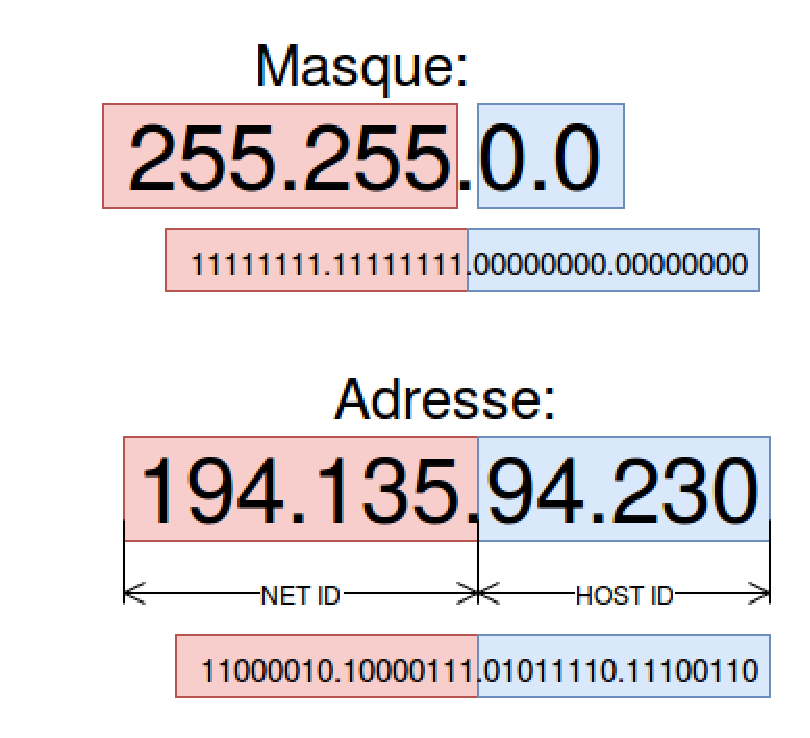
\includegraphics[width=7cm]{./pics/maskipv4.eps}
\caption{Example de masque de réseau.}
\label{fig:exmask}
\end{figure}

//TODO exemple
//TODO exemple invalide

\subsubsection{Classes d'adresse IP}
La technique de classe d'adressage IP ( classful network ) est une méthode
utilisée de 1981 à 1993 pour allouer des adresses IPV4.
Historiquement les classes d'adresse IP correspondaient à une plages d'adresses avec un masque figer pour une classe donnée.
Ce système permettait de déduire le masque en fonction
de l'adresse IP étant donné que chaque classe avait son masque défini de manière standard.
Il fut décrit dans le RFC 791\cite{url-RFC-791}.

Selon ce principe, chaque adresse IPv4 peut appartenir à une des 5 plages
d'adresses (appelées classes):

\begin{table}[h]
  \centering
% On paramètre ici le placement du texte dans les cases, en mode paragraphe de 5cm de large dans la case de gauche ("p{5cm}") et automatique avec un alignement à droite dans la case de droite ('r')
  \begin{tabular}{| p{5cm} | p{5cm} | r |}
    \hline
    \textbf{Classe} & \textbf{Masque reseau} & \textbf{Adresses}\\
    \hline
    A & 255.0.0.0 & De 0.0.0.0 a 127.255.255.255\\
    \hline
    B & 255.255.0.0 & De 128.0.0.0 a 191.255.255.255\\
    \hline
    C & 255.255.255.0 & De 192.0.0.0 a 223.255.255.255\\
    \hline
    D & 240.0.0.0 & De 224.0.0.0 a 239.255.255.255\\
    \hline
    E & Non defini & De 240.0.0.0 a 255.255.255.255\\
    \hline
  \end{tabular}
  \caption{Classes IPv4}
  \label{tab:classes}
\end{table}

A partir de ce tableau nous pouvons voir qu'il suffit de regarder les 4 bits de
poids fort pour déduire à quelle classe appartient une adresse.  Par exemple si
une machine à pour adresse 152.123.87.45 on sait en regardant les 4 premiers
bits que cette adresse fait partie de la classe B (car l'adresse commence par
10). De là, la machine n'a pas besoin de masque en plus car elle sait que le
masque correspondant un adresse de classe B est 255.255.0.0 .

Chaque classe à un certain nombre d'octets servants à identifier le réseau. Une
adresse IP de classe A à un identificateur de réseau sur 1 seul octet. Une
adresse IP de classe B sur 2 octet et une de classe C sur 3 octets.

Ce système permet donc d'adresser de nombreux réseaux avec un nombre de machine
variable en fonction de la classe, et tout cela sans avoir besoin de
communiquer ou de paramétrer un masque; celui-ci étant normalisé pour chaque
classe.  

Cependant il a un gros inconvénient, étant donné que les masques sont
figés, un réseau peut ne pas utiliser une partie plus ou moins importante
de ses adresses. Par exemple si un réseau contient 500 machines, il ne peut pas
utiliser d'adresse de classe A étant donné que celles-ci ne permettent d'avoir
que des réseaux de 254 machines maximum. Il va donc falloir utiliser des
adresses de classe B minimum, car elles permettent d'adresser 65534 machines au
sein d'un réseau\footnote{
De ce fait on remarque que la distribution de l’espace d’adressage entre
classes n'est pas homogène: la classe A a possédée 50\% de l’espace
d'adressage engendrée par les classes, la classe B 25\% , la classe C 12,5\%  et
les classes D et E 6,25\%.}. Nous pouvons donc utiliser 500 adresses sur les 65534
disponible, mais le reste sera "perdu".  Ce système était simpliste mais
n'était pas utilisable sur le long terme car il "gâche" des adresses en
n'utilisant pas tout son espace d'adressage.

Afin d'avoir un niveau supplémentaire, grâce auquel on gagne en flexibilité et
en efficacité dans l'attribution d'adresses à l'intérieur d'une classe, on a
introduit le concept de sous-réseau. Celui-ci correspond à couper la plage
d'adresses appartenant a un bloc d'une classe en plusieurs réseaux. Grâce aux
sous-réseaux on peut par exemple diviser une adresse de classe B en 256
sous-réseaux pouvant chacun avoir 256 interfaces connectées. 


\subsubsection{CIDR}

Aujourd'hui le système le plus utilisé est CIDR (Classless Inter-Domain
Routing) remplace le système de classe d'adresse. CIDR permet de créer des
masque beaucoup plus fin, étant donné qu'on n'est plus limité à des masque de
réseau fixe, on peut ajuster le masque pour avoir le nombre de machine
adressable dans un réseau le plus proche possible du nombre de machine que l'on
souhaite adressé.  Cela permet de limiter les pertes en adresse inutilisé, si
la plage est correctement découpée.  On peut donc créer des masques à la
séparation entre le NET ID et le HOST ID se trouve n'importe où, même en plein
milieu des octets (ce qui était impossible avec les classes d'adresse), ce qui
apporte une plus grande flexibilité.  Cela permet aussi de créer une hiérarchie
dans une plage d'adresse réseau qui serait découper en plusieurs réseaux
"fils", et cela permet notamment, avec cette hiérarchie, de réduire la table de
routage des routeur.  De là est né une nouvelle notation des masques: on écrit
le nombre de bit à 1 dans le masque à la suite de l'adresse IP et séparé par un
slash.


\begin{figure}[h]
\centering
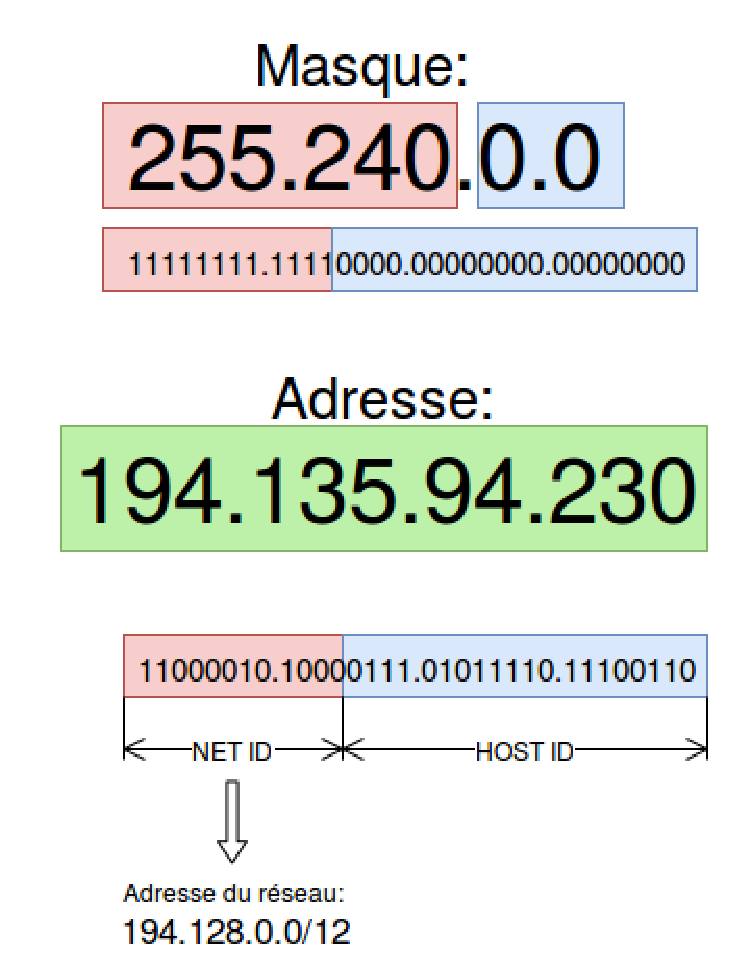
\includegraphics[width=7cm]{./pics/maskipv4cidr.eps}
\caption{Example de masque utilisant le systeme CIDR.}
\label{fig:exmask}
\end{figure}


\subsubsection{Types d'adresses}
La variété des exigences en matière de réseaux a donnée lieu à une
classification progressive des adresses selon des rôles bien précis. En effet,
pas toutes les adresses IPv4 ont la même signification: à certaines adresses
(ou plages d'adresses) ont été attribué par convention des fonctions ou des
caractéristiques particulières.  Dans la suite de cette partie nous analyserons les
adresses IP sous trois aspects différents: nous classifierons d'abord les adresses selon
le type de diffusion qu'elles permettent d'effectuer, puis nous introduirons le
concept d'adresse publique et d'adresse privée, enfin nous parlerons de l'utilisation
particulière qui a été faite avec certaines adresses.



\paragraph{Mode de diffusion}
Dans le cadre des transmissions, en plus de communiquer entre deux interfaces, il est 
parfois nécessaire qu'un message soit reçu par un groupe de machines ou que 
même la totalité du réseau reçoivent ce message.

On a défini pour cela plusieurs types de diffusions associés à certaines adresses particulières.

Le type de diffusion le plus utilisé est la diffusion en unicast. Dans ce mode,
l'adresse IP désigne une machine de manière unique. L'adresse IP appartient
à une seule machine et sert à l'identifier sur un réseau.  C'est le type
d'adresse que nous avons abordé jusqu'à présent.  Mais il peut être intéressant
de pouvoir contacter plusieurs machines en même temps. On pourrait bien sûr
envoyer des paquets en unicast à chaque machine que l'on souhaite contacter,
mais cela serait fastidieux et inonderait le réseau inutilement. Une solution plus
pratique est d'avoir une adresse qui désigne plusieurs machines à la fois. Cela
permet d'envoyer un seul paquet qui est remis à plusieurs machines. Il
existe pour faire cela plusieurs types de diffusion.
\begin{itemize}
\item Le broadcast: Ce mode de diffusion permet d'envoyer un paquet unique tout en 
joignant toutes les machines sur un réseau. Lorsque les machines reçoivent ce
paquet, elles s'aperçoivent que l'adresse de destination du paquet est l'adresse de
broadcast et elles vont alors traiter le paquet. L'adresse de broadcast d'un réseau
est défini comme la plus "haute" adresse du réseau: cela se traduit par la mise
à 1 de tous les bits de la partie HOST ID. Cette adresse ne peut donc pas être
attribuée à une machine en tant qu'adresse unicast.  Le broadcast est utilisé
par des protocoles tel que ARP et DHCP.  Nous pouvons remarquer qu'avec cette
définition, nous pouvons envoyer un message de broadcast à n'importe quel
réseau, incluant le notre. En réalité (sauf
configuration volontaire) les routeurs ne laissent pas passer les messages de
broadcast d'un réseau à un autre; excepté quelques cas spéciaux comme DHCP où un
serveur peut s'adresser à plusieurs réseaux, et où ses messages de broadcast
peuvent être relayés par les routeurs (appelés DHCP agents).
\item Multicast: Ce mode de diffusion permet d'envoyer un paquet à destination
de plusieurs machines. L'adresse IP multicast sera donc vu comme l'adresse d'un groupe
mutlicast, qui désigne donc plusieurs machines. Pour qu'une machine fasse partie d'un
groupe multicast, il faut qu'elle s'abonne à ce groupe: cela veut dire que si elle reçoit
un paquet avec comme adresse de destination l'adresse du groupe multicast, elle va traiter
le paquet.
Bien entendu les membres d'un même groupe ne sont pas obligés d'être sur le même réseau. Dans ce
cas les machines doivent indiquer à leur routeur qu'il existe un ou plusieurs groupe multicast et celui-ci deviendra alors un routeur multicast 
 Le protocole IGMP va entrer en jeu pour faire cet échange.
Cette indication a été rendu obligatoire dans le but de ne pas faire circuler tous les paquets a destination de groupes multicast.
 Il n'est en effet pas nécessaire de relayer tous les paquets de tous les groupes
multicast sur le réseau, si celui-ci ne contient aucun abonné au groupe.
Le faite d'avertir le routeur qu'il y a des machines abonnées à un groupe dans le réseau permet aussi à celui-ci
d'établir un lien avec l'émetteur. Mais ceci fait partie du routage des paquets par le routeur.
Il existe une plage d'adresse qui est réservée pour les adresses IP multicast. Lorsqu'on veut contacter
plusieurs machines, une adresse dans cette plage peut être utilisée.
Elle s'étend de l'adresse 224.0.0.0 à l'adresse 239.255.255.255 et a pour masque 240.0.0.0 . Cela laisse donc 2\^28 adresses
multicast différentes.
Au sein de cette plage d'adresse il existe une catégorisation:
//TODO
\begin{itemize}
\item
\end{itemize}
Ce mode permet de limiter le nombre de paquets envoyés pour joindre plusieurs machines et il est très utilisé dans le cas
de diffusions en streaming ou de vidéoconférences, où il faut faire parvenir une même information à plusieurs participants.

\item Anycast: Une adresse anycast, tout comme les adresse multicast, identifient plusieurs machines. La différence avec multicast
est qu'en mode de diffusion anycast, la paquet ne va pas être remit à tous les membre du groupe, mais seulement à un seul (le premier qui le réceptionne).
Le choix de la destination et le routage à adopter se base sur plusieurs critères telles que la "distance" avec la machine, la disponibilité,
la charge, ... . Cela permet d'avoir des systèmes toujours disponible même en cas de forte charge, en repartissant celle-ci sur
plusieurs machines.
\end{itemize}



\paragraph{Adresses publiques et adresses prive}
L'expansion exponentielle d'Internet a posé, seulement quelques années après sa création, des
soucis de pénurie d'adresses. Plusieurs mesures ont été prises pour limiter la
portée de ce problème. Malgré ça, le stock d'adresses IPv4 non réservée
est malheureusement épuisé depuis le 2011.

Une des dispositions les plus connues et efficaces a été la création du concept
d'adresses privées. Le RFC 1918 introduit la notion d'adresses privées: une adresse
appartenant à cet catégorie est un identifiant unique dans un réseau (ou sous
réseau) mais il ne comporte aucune contrainte d'unicité dans l'échelle globale
(Internet). L'idée derrière la conception des adresses privées était celle d'
avoir des identifiants qui peuvent être utilisés lorsque une machine n'a pas
pas besoin de communiquer avec des interfaces au-delà de son réseau.

A ce titre des plages d'adresses ont été réservées pour cet usage:

\begin{itemize}
\item Un bloc d'adresses appartenant a la classe A: \textbf{10.0.0.0/8}
\item 16 blocs d'adresses appartenant a la classe B: \textbf{172.16.0.0/12}
\item 256 blocs d'adresses appartenant a la classe C: \textbf{192.168.0.0/16}
\end{itemize}

\smallbreak
Le concept d'adresses privées s'oppose à celui d'adresses publiques: ce dernier est 
une adresse unique sur Internet et est en conséquence atteignable par n'importe
quel hôte sur Internet.

Aujourd'hui des systèmes comme celui de la NAT ({\it Network Address
Translation}) permettent à des machines ayant des adresses IP privée de communiquer
de manière transparente avec des hôtes en dehors de leur réseau. Ce système est
largement utilisé dans les réseaux domestiques pour permettre aux machines au
sein de ceux-ci d'être directement connecté à Internet. On parlera plus en
détail du NAT dans la section %TODO \ref{} %.
\smallbreak


 
L'augmentation des difficultés relatives à la procédure de réservation des adresses
publiques au sein des organisme responsables des allocations\cite{url-RFC-1918}
(tels que le IANA) ont contribués a promouvoir l'utilisation des adresses privées à la place
 des adresses publiques lorsque cela est possible.
L'utilisation des adresse privées a pour conséquence la préservation des plages
d'adresses IP publiques, ce qui constitue un avantage certain: l'utilisation
des adresses privées permet d'éviter le gaspillage des adresses publique là ou elles
ne sont pas nécessaires.


\paragraph{Adresses speciales}
L'usage spéciale d'une adresse IP découlait de l'émergence
%TODO (apparition??) 
d'un nouveau besoin dans le domaine des réseaux; c'est pour
ça que jusqu'à 2002, l'attribution des rôles spéciaux des adresses
IPv4 était présentés dans divers document, qui présentaient, et répondaient à chaque fois à une
problématique bien particulière. Le RFC3330 est un des premiers documents à
rassembler les classification des adresses IPv4 selon leur rôles et significations.

%TODO lien%

\begin{description}
\item[0.0.0.0/8]
Cette plage d'adresses indique la machine courante dans le réseau courant.
Les adresses dans cette plage sont notamment utilisées dans certains protocoles de
configuration comme adresse source, lorsqu'une machine n'a pas encore d'adresse effective.
%RFC 1122 %

\item[127.0.0.0/8]
Une adresse appartenant a ce bloc est dénommée adresse de {\it loopback}.  Un
paquet envoyé vers une telle adresse retourne directement chez l'expéditeur, sans sortir
du contexte de la machine émettrice. Parmi les adresses de cette plage,
127.0.0.1 est celle utilisée le plus fréquemment\footnote{Comme l'indique
le RFC 1122, certaines implémentations de l'adresse de {\it loopback} se
limitent à utiliser le bloc 127.0.0.1/32, ce qui se traduit par l'unique utilisation de
l'adresse 127.0.0.1 }: dans plusieurs contextes cet adresses est référencée par
l'alias "{\it localhost}".\footnote{La correspondance entre le nom {\it localhost} et
l'adresse 127.0.0.1 est généralement mise en place par le système d'exploitation.
Dans les systèmes de type UNIX une entrée reliant ces deux entités est généralement
présente dans le fichier "/etc/hosts".}
Une adresse de {\it loopback} n'a pas de sens en dehors
d'une interface même, et c'est pour cela qu'elle ne devrait apparaître à aucun moment dans le réseau.

%RFC 1122 %

\item[169.254.0.0/16]
Cet plage d'adresses a été désignée comme contenant les adresses qu'on appelle
de {\it lien local}.  Les adresses dites de {\it lien local} sont utilisée lorsqu'une 
machine n'a aucun moyen d'obtenir une adresse IP (par exemple par le biais
d'un serveur DHCP ou simplement avec une configuration manuelle).  L'obtention
d'une adresse de {\it lien local} est faite de façon automatique à travers un
processus d'auto-configuration souvent appelé par l'acronyme APIPA ({\it
Automatic Private Internet Protocol Addressing}) ou par le nom IPv4LL.  Le
fonctionnement du processus APIPA (décrit dans le RFC 3927) est assez complexe
 et entraîne l'utilisation de certaines fonctionnalités du
protocole ARP (qu'on traitera plus en détail dans la section %TODO \ref{sec:suiteproc} % )
. Son fonctionnement peut être synthétisé dans ses grandes lignes par la démarche suivante:

\begin{description}
\item[Sélection de l'adresse]
La machine choisit aléatoirement
    \footnote{Il est conseillé d'utiliser l'adresse MAC de l'interface en question
    pour générer l'adresse de {\it lien local} pour qu'il y ait une plus forte chance
    qu'elle soit unique dans le réseau.} 
une adresse appartenant à la plage 169.254.0.0/16

\item[Sondage sur l'adresse]
Une fois qu'on a sélectionné une adresse, il faut s'assurer que la même adresse ne soit
pas déjà utilisée par d'autres machines sur le réseau. Dans ce but la machine
pose la question à toutes les autres machines du réseau au moyen d'un ou plusieurs messages
en brodcast, et attend une réponse pendant un certain intervalle de temps\footnote{
Des précautions sont prises pour éviter les conflits générés par plusieurs
machines qui effectuent simultanément cette action pour la même adresse,
notamment: des intervalles de temps aléatoires entre l'envoie des messages et la mise
en place d'une écoute active des autres messages pendant le temps de l'enquête.}
L'absence de réponse indique que l'adresse est bien unique. Si l'adresse n'est
pas unique il faut en choisir une autre.

\item[Annonciation de l'adresse]
A ce point la machine peut communiquer aux autres machines l'adresse qu'elle
vient de réserver.

\end{description}



Ce processus est basé sur le concept de {\it Zeroconf}: il permet la mise en
place d'un réseau IPv4 sans aucune configuration. Ce type de système,
C'est aussi grâce a ce genre de systèmes, qu'on 
pourrait synthétiser par la devise %TODO slogan??  
"plug and play", que le concept de Networking (et avec lui Internet) a pu se
diffuser assez rapidement: grâce à APIPA un réseau IPv4 peut être facilement
mis en place sans le besoin d'aucune connaissance technique.\\

La plage d'adresses 169.254.0.0/16, désigne une plage d'adresse privée: les
adresses de type {\it lien local} ne sont donc pas atteignables en dehors de
leur réseau de définition. 
Cette plage d'adresses pose par contre des limites par rapport aux autres
plages d'adresses privée car, à la différence des autres, elle ne peut pas être
divisée en sous réseaux\footnote{Ce qui est assez logique si on considère que
le processus d'obtention d'une adresse de {\it lien local} (APIPA) utilise
les liens "physiques" entre les machines pour communiquer, et il ne peut
 considérer aucune notion de sous-réseau.}
: en effet un paquet destiné à une adresse de {\it lien local} ne doit pas être
retransmise par un hôte intermédiaire.\footnote{Dans le paquet destiné
a une adresse de {\it lien local} le champ TTL est usuellement mis a 1
pour empêcher des forwarding.}

\item[192.88.99.0/24]
Les adresses appartenant à ce bloc désignent des routeurs 
fournissant un service de type {\it 6to4}. Ce type de service
permet de relier des réseaux IPv4 avec des réseaux IPv6.
Les adresses dans cette plage sont traitées comme étant des adresses
de type {\it anycast}.


\end{description}




% Luigi Coniglio 
\subsection{En-tête IPv4}
Dans un paquet IPv4, les données utiles sont précédées par un en-tête ayant une longueur minimale de 20 octets 
(dans les cas où aucune option supplémentaire n'a été spécifiée).
La figure suivante montre le contenu de l'en-tête d'un paquet IPv4.

\begin{figure}[h]
\centering
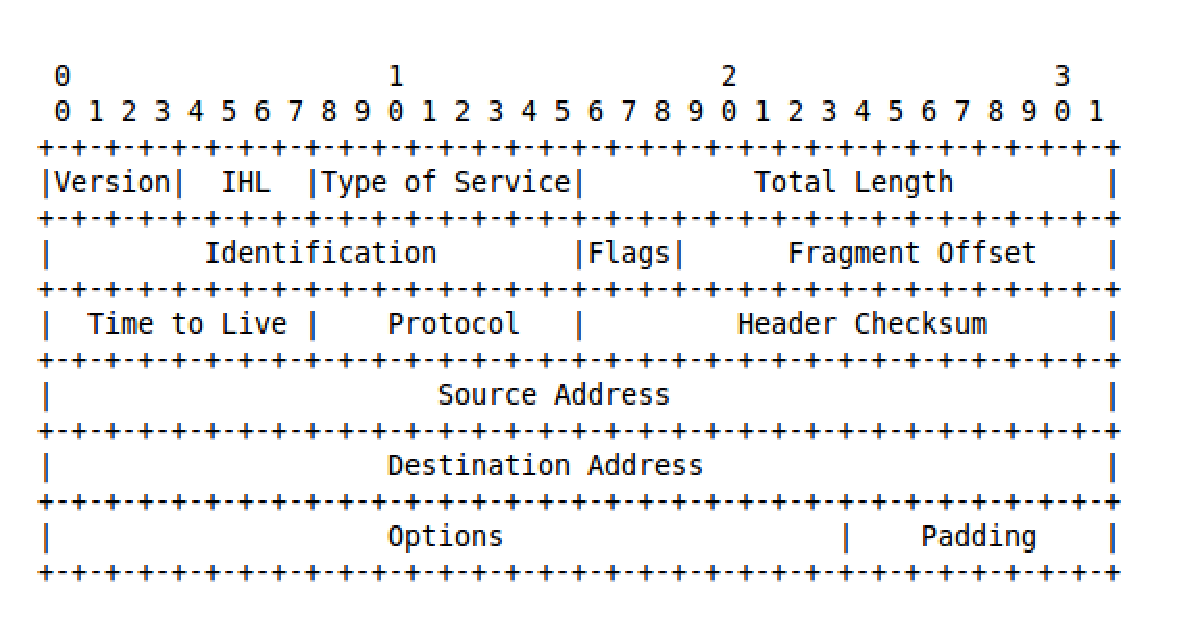
\includegraphics[width=12cm]{./pics/IPv4header.eps}
\caption{En-tete IPv4.}
\label{fig:entipv4}
\end{figure}


Comme on peut le voir sur la figure ci-dessus, un en-tête IPv4 est composé, en plus du padding, de
13 champs. En réalité nous verrons plus loin que cet en-tête
peut, quand c'est nécessaire, contenir un champ additionnel grâce auquel
on peut spécifier quelques options qui ne sont pas présentes dans les 13 champs
au dessus.


Commençons par voir en détail les 13 champs d'un en-tête IPv4 standard:

\begin{description}
\item [Version] 
Ce champ occupe les 4 premiers bits de l'en-tête IPv4.\\
Il est utilisé pour déterminer le type de protocole utilisé par la couche
réseau (couche 3). Dans le cas d'IPv4 ce champs contiendra la valeur
4, qui identifie le protocole IPv4.

Ce champ n'est pas positionné par hasard dans l'en-tête. En effet, pour
connaître la position des autres champs de l'en-tête, il faut d'abord savoir
quel est le protocole utilisé et donc le type de l'en-tête.
En pratique, dans la plupart des cas ce champ n'est pas très utile, car le
protocole à utiliser pour la couche 3 est souvent spécifié dans l'en-tête du
protocole de la couche liaison.

\item [IHL]
Le champ IHL (acronyme de Internet Header Length) spécifie la taille de l'en-tête IPv4. 
Bien entendu, en disant cela on souligne un concept important du protocole IPv4: 
la taille de l'en-tête n'est pas fixe.

La taille de l'en-tête est exprimée en blocs de 32 bits. Étant donné une taille de
4 bits pour le champ IHL, la longueur maximale d'un en-tête IPv4 est de 15 blocs de
32 bits, ce qui correspond à 60 octets. Comme l'en-tête IPv4 a une taille minimale
de 20 octets (160 bits), le champ IHL ne peut pas contenir une valeur inférieure à 5.

\item [Type of Service]
Le champ Type of Service, mieux connu sous l'acronyme ToS, est utilisé pour 
spécifier la qualité de service souhaité pour l'envoie d'un paquet IPv4.
Ce champ occupe un octet de l'en-tête et il est composé de trois parties.
Une première partie de 3 bits permettant d'indiquer la priorité avec laquelle
le paquet doit être traité, les 3 bits suivants sont utilisés pour spécifier 
certaines caractéristiques du service, notamment: le temps, le débit et la fiabilité.
Enfin, les deux derniers bits n'ont pas été utilisés et leur signification a été 
réservée pour des implémentations futures.

En réalité l'histoire de ces champs est bien plus longue et complexe,
car en pratique la façon d'utiliser ces champs a été modifiée plusieurs fois au 
cours du temps.
\footnote{L'utilisation des 8 bits du champ ToS a été redéfinie
par cinq standards différents (plus divers standards expérimentaux).
Les documents présentant ces standards sont mentionnés dans le chapitre 
"Historical Definitions for the IPv4 TOS Octet" du RFC 3168}
Ce manque de stabilité a parfois causé une certaine confusion lors des différentes implémentations.
\footnote{Comme le souligne le RFC 3260 {\it "At least one implementor has expressed confusion about the
relationship of the DSField, as defined in RFC 2474, to the use of
the TOS bits, as described in RFC 1349"}}

Aujourd'hui les 8 bits du champ ToS sont utilisés par le mécanisme DiffServ
(Differentiated Services). Ce système utilise les 6 bits premiers du champ
ToS (DSCP - Differentiated Services Code Point) pour marquer chaque paquet
comme appartenant à un niveau de priorité et à une classe de service. Chaque
classe détermine le type de traitement que doivent effectuer les routeurs sur le paquet qui le traverse
 (PHB - Per-Hop behaviour), toutefois le service offert
par chaque routeur est fortement lié à sa configuration.
\footnote {
{\it "The DiffServ standard does not specify a precise definition of "low," "medium,"
and "high" drop probability. Not all devices recognize the DiffServ (DS2 and
DS1) settings; and even when these settings are recognized, they do not
necessarily trigger the same PHB forwarding action at each network node. Each
node implements its own response based on how it is configured."} - 
Implementing Quality of Service Policies with DSCP
http://www.cisco.com/c/en/us/support/docs/quality-of-service-qos/qos-paquet-marking/10103-dscpvalues.html}
Les 2 derniers bits du champ ToS sont utilisés pour l'extension ECN ({\it Explicit Congestion
Notification }). Cette extension, proposée par le RFC2481n et introduite deux années plus tard par le RFC3168,
ajoute un système de contrôle de la congestion du trafic réseau. Dans le cas d'une saturation
du réseau, ce champ est utilisé pour notifier ce problème et demander au dispositif émetteur
une réduction du rythme auquel les paquets sont envoyés, afin de réduire l'attente et
la perte de paquets.

\item [Total length]
Comme le suggère son nom, ce champ est utilisé pour indiquer la taille totale du
paquet IPv4: en-tête + données. Le champ {\it Total length} est défini sur 16
bits, ce qui permet d'indiquer une valeur comprise entre 0 et 65 535 octets. Comme l'en-tête
est compris dans la longueur totale d'un paquet, cette valeur ne sera jamais inférieure
à 20 (taille minimale d'un en-tête IPv4 en octets).
Le RFC 791 impose à tous les dispositifs d'un réseau IPv4 la capacité de recevoir
des paquets d'une taille maximale de 576 octets, cette prérogative permet d'éviter une fragmentation excessive.

\item [Identification]
Ce champ (sur 16 bits) permet d'identifier les fragments appartenant au même paquet.

\item [Flags]
Les 3 bits du champ Flags sont utilisés pour gérer la fragmentation d'un paquet.
Un de ces bits est utilisé pour indiquer si le paquet peut être fragmenté ou
non. Ce bit, appelé DF ({\it Don't Fragment}), doit être pris en considération
par les routeurs sur le chemin du paquet pour décider si un paquet est trop grand pour être
transmit, s'il doit être retransmit sous forme de fragments plus petits ou s'il doit être rejeté. 
Un autre bit, appelé MF ({\it More Fragments}), indique si le paquet est suivi 
par d'autres fragments. Le bit MF est mis à 0 dans le dernier fragment ou dans
les paquets qui n'ont pas été fragmentés.

Un des trois bits de ce champs n'est pas utilisé actuellement mais il a été
réservé pour de possibles applications futures.
\footnote {Ce bit a aussi été le protagoniste d'un des plus connu poissons
d'avril de l'IETF. Pour faciliter les tâches des systèmes de filtrage 
le RFC 3514 propose d'utiliser ce bit pour étiqueter les paquets malveillants et à ce
titre tous les paquets étant envoyés avec ce bit (renommé "{\it Evil Bit}") 
mis à 1 seraient mis à la poubelle.}

\item [Fragment Offset]
Lorsqu'un paquet a été fragmenté, cet en-tête est utilisé pour déterminer la
position (offset) d'un fragment par rapport à l'ensemble du paquet réassemblé.
Le décalage de chaque fragment est exprimé en blocs de huit octets (ou 64
bits). Le champ Fragment Offset utilise 13 bits de l'en-tête IPv4, ce qui permet
un offset maximale de 65528 octets.\footnote {En pratique un tel offset n'est
jamais utilisé car, en ajoutant un en-tête minimale de 20 octets, la taille
totale du paquet réassemblé dépasserait la longueur maximale d'un paquet IPv4.}
Étant donné que le flag MF ({\it More Fragments}) doit être mis à zéro lorsqu'un paquet 
n'est pas fragmenté, ou si il est le dernier fragment d'un paquet plus grand, 
l'unique différence entre ces deux types de paquets est la valeur du 
champ Fragment Offset qui, dans le cas d'un paquet non fragmenté, est
toujours zéro.

\item [Time to Live]
Ce champ détermine le nombre maximal de fois qu'un paquet peut être retransmit. 
Il est utilisé pour empêcher qu'un paquet puisse être retransmit à l'infini.
Chaque routeur le long du chemin d'un paquet regarde la valeur du champ. Si celle-ci
a atteint 0, il détruit le paquet, et sinon il décrémente le champ par le
nombre de secondes que le paquet passe en attente avant qu'il soit transmis.

En théorie, le TTL indique le nombre de secondes pendant lesquelles un paquet
peut continuer à être retransmis dans un réseau, mais un routeur 
 décrémente toujours ce champ d'au moins 1 (même si le paquet a été
retransmis en moins d'une seconde) et, en considérant les performances des routeurs
d'aujourd'hui, le TTL indique en pratique le nombre maximum de routeur qu'un paquet
 peut traverser au cours de son acheminement.

L'espace réservé au TTL dans l'en-tête IPv4 est d'un octet, ce qui veut dire qu'on a un 
TTL maximum de 255.\footnote {Le RFC 1700 recommande une valeur par défaut de 64.}

Quand un paquet a été détruit suite à l'expiration du TTL, le routeur qui a
détruit le paquet peut décider d'envoyer un message d'erreur à l'émetteur du
paquet détruit. Ce type de message (ICMP Time exceeded) est également utilisé comme
outil par {\it traceroute} pour découvrir, approximativement, le chemin 
d'un paquet IP.

\item [Protocol]
Chaque paquet IPv4 spécifie le protocole utilisé par les données transmises:
cela est l'objectif de ce champs de 8 bits 

\item [Header Checksum]
Ce champ contient une somme de contrôle et est utilisé pour détecter des 
erreurs dans l'en-tête IPv4. La valeur de ce champ est recalculé à
chaque retransmission\footnote {Cela est nécessaire car le TTL est décrémenté
à chaque retransmission et un changement de l'en-tête amène à une valeur différente
dans la somme de contrôle}: si la somme de contrôle ne correspond pas avec celle 
présente dans l'en-tête du paquet, celui-ci est détruit.


\item [adresse source et adresse destination]
Les adresses de chaque paquet IPv4 (soit l'adresse source et l'adresse de
destination du paquet) sont représentés sous forme d'une suite de 32 bits.

L'adresse source de chaque paquet représente dans la plupart des cas
l'adresse logique\footnote {Il ne faut surtout pas oublier la différence entre
une adresse physique, comme par exemple une adresse MAC (qui est liée a
l'hardware et est donc unique pour chaque machine), et une adresse logique,
comme par exemple une adresse IP (qui peut changer et identifie une machine
dans un réseau en particulier).} de la machine qui a envoyé le paquet
(à laquelle il faudra donc éventuellement répondre).  Dans certains cas,
 cette adresse ne correspond pas à celle de la machine qui a envoyé
le paquet, c'est par exemple ce qui se passe dans une requête, {\it ARP probe}
%TODO to correct: 0.0.0.0 symbolise la machine actuelle%
lorsque la valeur de l'adresse de la machine source est 0.0.0.0 (ce qui représente
une adresse indéfinie\footnote {La signification de l'adresse 0.0.0.0
est liée à la façon dont elle est utilisée. En général elle indique {\it aucune
adresse en particulier}. 

Dans la plupart des cas, cette adresse est utilisée
pour indiquer une de ces valeurs: l'adresse de la machine courante (c'est
l'adresse de loopback), n'importe quelle adresse ou le réseau (c'est le cas de la
route par défaut dans une table de routage), une adresse indéfinie ou bien une
combinaison des possibilités précédentes (c'est le cas d'une requête {\it ARP
probe} ou bien d'une requête {\it DHCP Discovery} ou {\it DHCP Request}, où
 l'adresse source 0.0.0.0 indique une adresse indéfinie mais aussi l'adresse
de la machine actuelle, qui par ailleurs n'est pas encore défini...).}
) car elle n'a pas encore déterminée son adresse IP. 

L'adresse de destination d'un paquet IPv4 identifie la machine vers
laquelle le paquet doit être expédié. Comme dans le cas de l'adresse source,
 l'adresse de destination peut aussi contenir des valeurs spéciales. En effet, certaines 
valeurs peuvent être utilisée par exemple pour identifier plusieurs machines
(adresses multicast), toutes les machines d'un réseau (adresse de broadcast) ou
la machine actuelle (adresse de loopback).

Une description plus détaillée des mécanismes liées aux adresses IPv4 est
proposée dans le chapitre  
%TODO mettre chapitre% 
de ce rapport.


\item [Options] 
Ce champ n'est pas obligatoire et il peut donc ne pas être présent dans un
en-tête IPv4. La présence de ce champ est déterminé par la valeur de
l'IHL: lorsque cette valeur indique une taille de l'en-tête IPv4 supérieure à 
la taille minimale (20 octets), l'en-tête contient des options.
Étant donné qu'un en-tête IPv4 peut avoir une taille maximale de 
60 octets (la valeur du IHL est égal à 15), le champ Options peut occuper
40 octets au maximum.

Ce champ a été conçu pour étendre les possibilités d'IPv4 en ajoutant des fonctions
supplémentaires.  Aujourd'hui il y a quelques dizaines d'options qui ont été
spécifiées\cite{url-optsIPv4} (si on considère également les options expérimentales)
mais peut d'entre elles sont réellement utilisées. Parmi les options les plus connues
on retrouve par exemple des ajouts utiles à l'administration et au debuggage
d'un réseau, comme {\it Record route} qui permet d'enregistrer les adresses
des routeurs dans le chemin d'un paquet IP, et {\it Timestamp} qui permet de
savoir le temps passé entre chaque saut du chemin.

Parmi les options il en y a deux qui ont une fonction spéciale: EOL 
({\it End Of Option List}) et NOP ({\it No Operation}): l'option EOL 
est utilisée pour indiquer la fin de la chaîne d'options, NOP est une option
sans aucun effet, elle est utilisée comme remplissage pour aligner les options 
quand elles ne sont pas alignées sur 4 octets\footnote {On rappelle que 
le champ IHL indique la longueur de l'en-tête IPv4 en blocs de 32 bits 
(4 octets)}.



\item [Padding] 
Le padding ne contient que des zéros et est utilisé quand la fin de l'en-tête
n'est pas aligné sur 32 bits (4 octets). Bien entendu, ce champ est optionnel:
en effet, il est seulement nécessaire lorsque l'en-tête IPv4 termine avec
une option dont la limite n'est pas alignée sur 32 bits. Un en-tête d'un paquet IPv4 
de 20 octets (donc sans aucune option) n'a besoin d'aucun Padding car il est aligné sur
4 octets (20 étant un multiple de 4).
\end{description}

\subsection{Routage}

Nous avons vu comment les machines était adressées, de quoi était constitué les
paquets IPv4 et comment elles pouvaient communiquer entre elles.  Nous avons
donc maintenant des réseaux constitués d'une ou plusieurs machine, mais ces
réseaux sont indépendant et totalement hermétique les uns les autres. Il
pourrait être intéressant de pourvoir faire communiquer ces réseaux entre eux.
C'est le but du routage que de faire passer des paquets d'un réseau à un autre.

\subsubsection{Principe du routage}

\paragraph{Materiel}
Le routage est une action qui va être délégué à une machine servant à établir
un lien entre deux ou plusieurs réseaux.  Le matériel qui va s'occuper de faire
cela est appelé un routeur: cela peut être n'importe quel ordinateur configuré
pour faire du routage, ou dans la plupart des cas une machine "dédié", celle-ci
étant conçu pour le routage et ayant des caractéristiques adaptée a cette tache
(nombre des interfaces réseaux, consommation réduite, accélération matérielle, ... ).

Comme un routeur se charge de faire de liaison entre différents réseaux, il doit
forcément avoir deux ou plusieurs interfaces réseaux: au moins une pour chaque
réseau qui doit lier.

\paragraph{Table de routage}
Afin que le routeur puisse envoyer un paquet vers sa destination, il faut qu'il
sache vers quelle direction transmettre le paquet pour qu'il soit sur le bon
réseau. Il faut pour cela qu'il ait une table regroupant les associations entre
les réseaux et la direction vers laquelle ils se trouvent: cette table est
appelée table de routage.  Cette table de routage peux être rempli de plusieurs
manières: soit manuellement par l'administrateur réseau (le réseau est donc
figé et n'est pas tolérant aux pannes), soit dynamiquement à l'aide de
protocole de routage (RIP, OSPF, BGP, IS-IS,...) qui vont modifier en temps
réel la table de routage pour s'adapter au changement du réseau et être
tolèrent aux pannes.

Lorsque des hôtes d'un réseau ont besoins de contacter un autre réseau pour le
biais d'un routeur, ils vont également utiliser une table de routage.  En
effet, lorsqu'un hôte veut envoyer un paquet vers un autre réseau, il faut
qu'il ai l'adresse du routeur auquel envoyer sont paquet pour que celui-ci le
transmette en direction du bon réseau.

\paragraph{Forwarding}

Lorsqu'un routeur reçoit un paquet qui ne lui ai pas destiné il va utiliser
l'entré de sa table la plus précise pour joindre le réseau de destination.

Pour faire cela il essaye de déterminer quel NET ID de sa table de routage
correspond le plus à l'adresse destination.  Une fois trouvé, il va transmettre
le paquet vers la direction associé à celui-ci.
Cette direction peux être:
\begin{itemize}
\item Soit être une interface: dans ce cas le réseau en question se trouve
directement derrière cette interface. Il faut donc envoyer le paquet
directement à son destinataire.
\item Soit une adresse IP: qui désigne l'adresse du prochain routeur auquel il
faut envoyer le paquet et qui va s'occuper à son tour de diriger le paquet vers
sa destination.
\end{itemize}

\subsubsection{Routage en IPv4}
\paragraph{Agrégation CIDR}
L'adressage avec masque CIDR à permis de réduire la taille de la table de
routage en agrégeant plusieurs entrées en une seul; ce qui était impossible avec
l'utilisation de classes d'adresses.  En effet, avec des classes d'adresses, le
masque étant fixé et les classes ne se chevauchant pas, il n'était donc pas
possible de créer une hiérarchie dans entre les réseaux.  Ainsi il n'est pas
possible d'agréger plusieurs réseaux en une seule entrée dans la table de
routage.

\begin{figure}
\centering
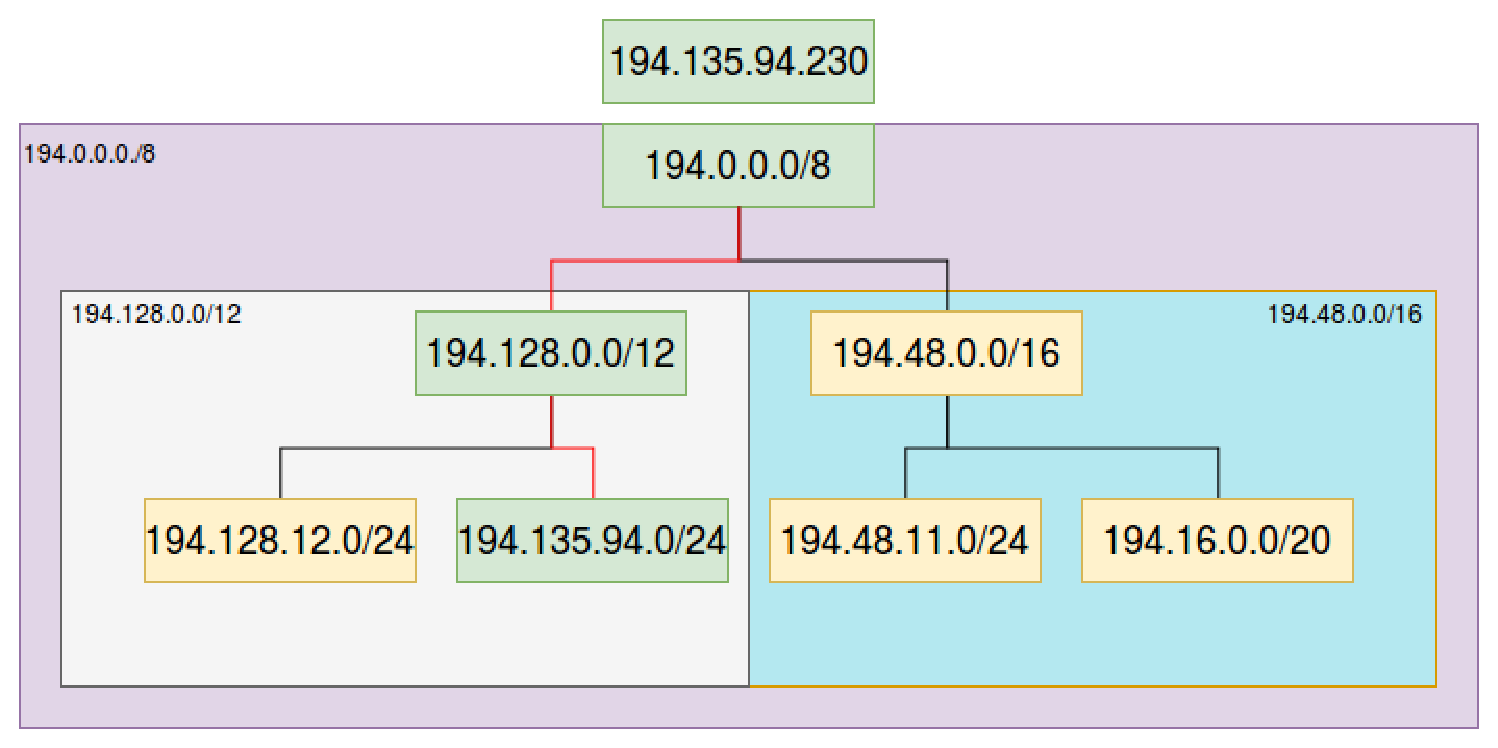
\includegraphics[width=15cm]{./pics/routagecidr.eps}
\caption{Agregation des adresses reseau base sur leur hierarchie}
\label{fig:routcidr}
\end{figure}

L'adressage avec un masque CIDR permet d'être totalement libre dans le choix du
masque. Ceci permet de créer une hiérarchie dans entre les réseaux. De ce fait,
un routeur n'est pas obligé de créer une entrée pour chaque réseaux dans la
table de routage mais, quand il est possible, il créera seulement une entrée
comme étant l'agrégation des réseaux sous-jacent représenté par l'entrée.

\paragraph{Adresses spéciales}

Comme nous l'avons vu plus haut, certaines adresses sont utilisé pour des
tâches particulières. Cela peut induire un traitement particulier lors du routage
d'un paquet.  C'est la cas par exemple des adresses de {\it lien local} qui ne
peuvent jamais traverser un routeur pour joindre un réseau différent. En effet
les adresses de lien local sont propre à un réseau.
Un autre cas ou les adresses sont limitées, est le cas des adresses de broadcast.
En temps normal, les routeurs bloques les paquets émis en broadcast, de sorte qu'il ne se propage pas en dehors du réseau d'origine. Il est facile d'imaginer les problèmes que causerai un paquet émis en broadcast sur Internet. Une exception étant les paquets DHCP émis en broadcast et qui traverse les routeurs par le biais des agents DHCP.
Un dernier cas particulier sont les adresses privées: le routage des paquets ayant une adresse privée en destination n'a pas de sens en dehors d'un réseau privé. Les adresse privées peuvent passer les routeurs et avoir du sens du moment qu'elle reste dans un réseau privé.

